\documentclass[aspectratio=169]{beamer}

\usepackage[utf8]{inputenc}
\usepackage{soul}
\usepackage{pdfpcnotes}
\usepackage{listings}
\usepackage{tikz}
\usepackage{booktabs}
\usepackage{minted}

\usetheme{Hannover}
\usecolortheme{dove}

\AtBeginSection[]{
  \begin{frame}
  \vfill
  \centering
  \begin{beamercolorbox}[sep=8pt,center,shadow=true,rounded=true]{title}
    \usebeamerfont{title}\insertsectionhead\par%
  \end{beamercolorbox}
  \vfill
  \end{frame}
}

\lstset{language=C++,
                basicstyle=\ttfamily,
                keywordstyle=\color{blue}\ttfamily,
                stringstyle=\color{red}\ttfamily,
                commentstyle=\color{purple}\ttfamily,
                morecomment=[l][\color{magenta}]{\#}
}


\title{Eine Einführung in modernes C++ mit CMake}
\author{Paul Nykiel}
\date{\today}

\begin{document}
\maketitle

\frame{
    \pnote{Sofort Fragen!}
    \pnote{Feedback erwünscht}
    \tableofcontents
}

\section{Einleitung}
\begin{frame}
    \frametitle{Was ist C++}
    \pnote{Kurz Hintergrund für Einordnung}
    \begin{itemize}
        \item \st{C with classes}
            \pnote{Ursprünglicher Name, da initial nur Erweiterung von C um Objektorientung}
            \pause
        \item Standardisiert und offen
            \pnote{Viele Compiler, Gute Dokumentation,  Entscheidungen werden im Komitee getroffen, nicht von einzelnen Firmen}
            \pause
        \item Wird in quasi jeder Domäne genutzt
            \pnote{Embedded, Betriebssysteme, Systemnahe Entwicklung, Signalverarbeitung (Codierung), Desktop-Anwendungen, Spiele, Server-Anwendungen, HPC...}
            \pause
        \item Ziele: Performanter und sicherer Code
            \pnote{Sicheres Typensystem, checks zur Compile Time (unterschied zur Run Timer hervorheben), maschinennah}
    \end{itemize}
\end{frame}

\begin{frame}
    \frametitle{C++ im Vergleich zu Java}
    \begin{itemize}
        \item Undefiniertes Verhalten 
            \pnote{Null-Pointer, fehlendes Return, division durch Null. Kann nicht vom Compiler kontrolliert werden und zur Runtime gibt es keine passnden Mechanismen  z.B. Microcontroller. Aber quasi jede Sprache hat undefiniertes Verhalten bezeichnet es aber nicht so (z.B. Race-Conditions)}
            \pause
        \item Keine automatische Speicherverwaltung 
            \pnote{Keine Aufgabe der Sprache, wenn benötigt liefert die STL passende Container. Bei Microcontroller oder Echtzeitanwendungen nicht gewünscht.
            Unterscheidung Heap und Stack hervorheben.}
            \pause
        \item Kleiner Sprachkern und kleine Standardlibrary 
            \pnote{60 Schlüsselwörter, C\# z.B. 86. Keine UI, kein Networking...}
            \pause
        \item Templates 
            \pnote{Nicht generics, viel mächtiger, z.B. Boost MSM, sichere Pointer (Guideline support library), Turing-vollständig}
            \pause
        \item Operatorenüberladung
            \pnote{Bsp. Vektor, Iteratoren...}
            \pause
        \item Tendentiell weniger tiefe Vererbung
            \pnote{Z.b. Container und Iteratoren, keine Überklasse aber Eigenschaften (forward-Iterator), dadurch weniger Boilerplate}
            \pause
        \item Mehrfachvererbung
            \pnote{Dadurch keine Interfaces notwendig, aber selten genutzt}
            \pause
        \item Definierte Objektlebenszeit
            \pnote{Konstruktor, Destruktor, Scope}
    \end{itemize}
\end{frame}

\section{Ein erstes C++ Programm}

\begin{frame}
    \Huge{Beispiel: Hello World}
    \pnote{Hello World. Erklärung: include, keine main-Klasse, namespaces, Operatorenüberladung, Vergleich Code-Länge mit Java}
\end{frame}

\begin{frame}
    \frametitle{Vom Sourcecode zur ausführbaren Datei}
    \begin{columns}
        \begin{column}{.5\textwidth}
            \begin{itemize}
                \item<+-> Präprozessor 
                    \pnote{Erklärung include und define an Hello World Bsp (gcc -E), einfache Textersetzung, Erklärung an Tafel}
                \item<+-> Compiler 
                    \pnote{Übersetzten von der Übersetzungseinheit in Assemblercode, Übersetzungseinheit definieren}
                \item<+-> Linker 
                    \pnote{Baut Programm zusammen und sucht Funktionen in anderen Übersetzungseinheiten}
                \item<+-> \lstinline{\#include}s sichern Typkonsistenz
                    \pnote{Unterschied Definition und Deklaration, Doku im Header gut für Übersicht}
                \item<+-> Templates müssen im Header definiert werden
                    \pnote{Compiler muss alle instanziierungen kennen, langsamer Buildprozess}
            \end{itemize}
        \end{column}
        \begin{column}{.5\textwidth}
            \begin{figure}
                \includegraphics[width=\textwidth]{build.pdf}
            \end{figure}
        \end{column}
    \end{columns}
\end{frame}

\begin{frame}
    \Huge{Beispiel: Eine zweite Übersetzungseinheit}
    \pnote{Zweites Cpp File, alles einfach in g++ schmeißen,
    Message als std::string (nicht ref)}
\end{frame}

\section{CMake}

\begin{frame}
    \frametitle{Warum ein Buildsystem}
    \begin{itemize}
        \item Nur geänderte Dateien neu kompilieren 
            \pnote{erkennt welche Files geändert wurde, größere Projekte kompilieren sonst jedes mal mehrere Minuten bis Stunden}
            \pause
        \item Einzelner Befehl an Compiler wird zu kompliziert
            \pnote{Vor allem bei vielen Flags und vielen Dateien}
            \pause
        \item Portabilität
            \pnote{Compiler und Flags werden unnabhängig vom Os und von installierten Compilern angegeben}
    \end{itemize}
\end{frame}

\begin{frame}
    \frametitle{CMake}
    Wird durch Datei \lstinline{CMakeLists.txt} konfiguriert:
    \inputminted{cmake}{examples/slides/CMakeLists.txt}
\end{frame}

\begin{frame}
    \Huge{Beispiel: CMake}
    \pnote{Einfaches CMake File dazu bauen, nochmal kompilieren, Lib ändern zeigen dass main nicht neu gebaut wird}
\end{frame}

\section{Mehr C++}

\begin{frame}
    \frametitle{Speicherverwaltung}
    \begin{itemize}
        \item \lstinputlisting{examples/slides/copy.cpp}
            \pnote{f ist Funktion list->list und b ist list. Was passiert hier, wie viele Objekte existieren, wie viel Speicher wird genutzt, wie oft wird kopiert}
            \pause
        \item Jegliche Zuweisung ist eine Kopie, auch für Funktionsargumente
            \pnote{Funktionsargumente, Zuweisung.... Explizit große Container erwähnen}
            \pause
        \item Einfach verständlich
            \pnote{Vgl. komisches Java Verhalten. Trivial ein Objekt zu kopieren, deep copy in Java und C\# schwierig (Internet: selber implementieren oder serializieren und deserializieren)}
            \pause
        \item Für große Objekte unnötige Performanceeinbuße
            \pnote{Spricht gegen das was ich in Einleitung gesagt habe, Performance in C++ wichtig}
    \end{itemize}
\end{frame}

\begin{frame}
    \frametitle{Pointer}
    \begin{itemize}
        \item Pointer 
            \pnote{"Vererbt" von C}
            \pause
        \item Angst!
            \pause
        \item Gefährlich!
            \pause
        \item Böse!
            \pnote{Pointer kurz erklären, kurz Owner (malloc/new) bzw. nur als Referenz erklären}
            \pause
        \item Nicht schlimm aber viel Fehlerpotential
            \pnote{Leaks, Owner nicht definiert, vor allem bei Librarys relevant}
            \pause
        \item \lstinline{int b = 17; int *a = &b;}
            \pnote{Pointer als Referenz}
            \pause
        \item \lstinline{int *c = new int();}
            \pnote{Pointer als Owner, Hier gleich ein potentieller Leak}
            \pause
        \item \lstinline{delete c;}
            \pnote{Immer mit delete, das will doch wirklich keiner}
            \pause
        \item Gehört nicht in die Anwendungslogik
            \pnote{Permanente Fehlerquelle, Zeitverschwendung, Ab jetzt als Raw-Pointer bezeichnet und nie wieder verwenden!}
    \end{itemize}
\end{frame}

\begin{frame}
    \frametitle{Stack und Heap}
    \begin{columns}
        \begin{column}{.5\textwidth}
            \begin{itemize}
                \item<+-> Hauptspeicher (RAM) wird aus zwei Richtungen vergeben
                    \pnote{Aufteilung in Stack für Performance und Heap für dynamischen Speicher}
                \item<+-> Stack wird für Funktion aufgebaut
                    \pnote{Schnell da FILO, wird automatisch wieder abgebaut}
                \item<+-> Heap für dynamischen Speicher
                    \pnote{Langsam, freier Speicher muss erst gefunden werden}
                \item<+-> Speicher auf dem Heap muss händisch reserviert und freigegeben werden
                    \pnote{Memory Leak wenn nicht wieder freigegeben}
                \item<+-> Bei mehr als einem Owner Verwaltung kompliziert
                    \pnote{Owner: Funktion die Pointer kennt}
            \end{itemize}
        \end{column}
        \begin{column}{.5\textwidth}
            \begin{figure}[H]
                \centering
                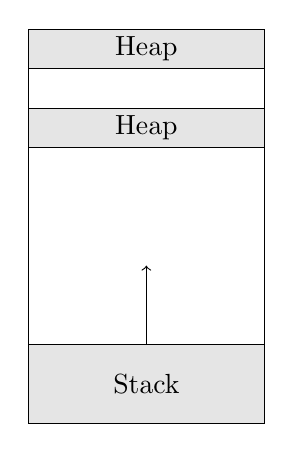
\begin{tikzpicture}
                    \draw [draw] (0,0) rectangle (3,5);
                    \filldraw [draw=black,fill=gray!20] (0,0) rectangle (3,1) node[pos=.5] {Stack};
                    \filldraw [draw=black,fill=gray!20] (0,4.5) rectangle (3,5) node[pos=.5] {Heap};
                    \filldraw [draw=black,fill=gray!20] (0,3.5) rectangle (3,4) node[pos=.5] {Heap};
                    \draw [->] (1.5,1) -- (1.5,2);
                \end{tikzpicture}
            \end{figure}
        \end{column}
    \end{columns}
\end{frame}

\begin{frame}
    \frametitle{Beispiel Pointer}
    \lstinputlisting{examples/slides/pointer.cpp}
    \pnote{Auf Stack: Kein Owner}
    \pnote{Auf Heap: Owner}
\end{frame}

\begin{frame}
    \frametitle{Smart-Pointer}
    \begin{itemize}
        \item Standardlibrary kann Verwaltung übernehmen
            \pnote{Erwähnung Operatorenüberladung und Lifetime}
            \pause
        \item \lstinline{unique\_ptr}
            \pnote{Quasi Drop-In-Replacement für Raw-Ptr, machen selber den Speicher am Ende der Lebenszeit frei}
            \pause
        \item Genau ein Owner
            \pnote{Explizit verboten zu kopieren (=delete), Bsp. kopieren in Klasse, jetzt uneindeutiger Owner. Oftmals für Factory Methoden, kein Overhead zu Raw-Pointer}
            \pause
        \item
            \lstinline{std::unique\_ptr<int> a = std::make\_unique<int>(17);}
            \pause
        \item \lstinline{shared\_ptr}
            \pnote{Zusätzlich Zählen von Instanzen (siehe Copy-Constructor)}
            \pause
        \item Quasi immer nutzbar
            \pnote{Dafür kopieren... minimal langsamer (nicht bei Zugriff)}
        \item
            \lstinline{std::shared\_ptr<int> a = std::make\_shared<int>(17);}
    \end{itemize}
\end{frame}

\begin{frame}
    \frametitle{Referenzen}
    \begin{itemize}
        \item Sprachfeature kein Library-Feature
            \pnote{Werden vom Compiler zu Pointern gemacht, nie Owner. Hier betrachtet L-Value-Referenzen}
            \pause
        \item Können nicht null sein
            \pnote{Zeigen immer auf anderes Objekt, eine Art Alias}
            \pause
        \item Können aber ungültig werden
            \pnote{z.B. lokale Variablen}
            \pause
        \item
            \lstinline{int b = 17; int &a = b;}
    \end{itemize}
\end{frame}

\begin{frame}
    \frametitle{Zusammenfassung Pointer}
    \begin{itemize}
        \item Raw-Pointer: Sollten quasi nie verwendet werden
            \pnote{Ausser pre C++11 und mit C APIs}
            \pause
        \item Unique-Pointer: Oftmals ersatz für Raw-Pointer
            \pnote{Limitierung: Ein Owner kein Overhead}
            \pause
        \item Shared-Pointer: Sichere Pointer für beliebig viele Owner
            \pnote{Am Ähnlichsten zu Java, aber etwas Overhead (immer noch weniger als Java und definierte Lifetime)}
            \pause
        \item Referenzen: Oftmals um Kopien zu vermeiden
            \pnote{Sprachfeature}
    \end{itemize}
\end{frame}

\begin{frame}
    \Huge{Beispiel: Pointer \& Referenzen}
    \pnote{Wo Pointer/Ref einbauen? Frage welche Sorte Pointer. HelloWorld Lib Ergänzen mit Referenzen, jetzt in CLion}
\end{frame}

\section{Design Pattern}

\begin{frame}
    \frametitle{Const-Correctness}
    \begin{itemize}
        \item Alles per Referenz: Super Effizient aber Fehlerquelle
            \pnote{Beispiel: ausversehen einfügen in Map, allgemeine Fehlerquelle immer nur minimale Rechte, Dokumentation}
            \pause
        \item Const-Referenzen
            \pnote{Ergänze Beispiel}
            \pause
        \item \lstinline{const int &a = b;}
            \pnote{Read-Only "nur anschauen"}
            \pause
        \item Const-Memberfunktionen
            \pnote{Beispiel getter}
            \pause
        \item \lstinline{int getX() const \{...}
            \pnote{Const am ende der Definition this ist in der Funktion konstant}
            \pause
        \item \lstinline{mutable}
            \pnote{Beispiel Log}
    \end{itemize}
\end{frame}

\begin{frame}
    \Huge{Beispiel: Const-Correctness}
    \pnote{const einfügen hello world}
\end{frame}

\begin{frame}
    \frametitle{RAII}
    \begin{itemize}
        \item Resource acquisition is initialization
            \pnote{Fehlerreduktion, Einfachheit, Exception Safety}
            \pause
        \item Objekt akquiriert Resourcen im Konstruktor und gibt sie im
            Destruktor frei
            \pnote{Bsp. Datei, Mutex, Vector. Vgl try catch finally java}
            \pause
        \item
            \lstinputlisting{examples/slides/raii.cpp}
            \pnote{Trailing return type, Const-Correctness, Objekte werden im Konstruktor initialisiert, alle Objekte werden im Konstruktor geschlossen} 
    \end{itemize}
\end{frame}

\section{OOP in C++}

\begin{frame}
    \frametitle{Klassendeklaration}
    \lstinputlisting{examples/slides/class.h}
    \pnote{Hinweis unterschied Deklaration und Definition. Vererbung, Sichtbarkeit von Vererbung, public, private, Konstruktor, Trailing return type, const Const-Correctness}
\end{frame}

\begin{frame}
    \frametitle{Klassendefinition}
    \lstinputlisting{examples/slides/class.cpp}
    \pnote{Initializierung in Braced-Initializer, Super-Konstruktor, this als Pointer}
\end{frame}

\begin{frame}
    \frametitle{Namespaces}
    \lstinputlisting{examples/slides/namespace.cpp}
    \pause
    \begin{itemize}
        \item Struktur
            \pause
        \item Keinen Einfluss auf Sichtbarkeit
            \pause
        \item Namespaces nicht mit \lstinline{using} einbinden
            \pnote{Beispiel std::distance}
    \end{itemize}
\end{frame}

\begin{frame}
    \Huge{Beispiel: HelloWorld OOP}
\end{frame}

\section{Noch mehr C++}

\begin{frame}
    \frametitle{Casts und Null-Pointer}
    \begin{itemize}
        \item \lstinline{static\_cast<T>(a)}
            \pnote{Castet Typen in kompatible Typen (hier von a nach T), kompatibilität wird zur Compile Time gecheckt}
            \pause
        \item \lstinline{dynamic\_cast<T>(a)}
            \pnote{Castet zur Runtime, vor allem für Pointer und Polyphormismus, kann Null sein}
            \pause
        \item \lstinline{0}, \lstinline{NULL} und \lstinline{nullptr}
            \pnote{Abstammung aus C, Erklärung mit Überladung}
            \pause
        \item Trailing \lstinline{return}-type 
            \lstinputlisting{examples/slides/trailingreturn.cpp}
            \pnote{Mathematische Notation, oftmals einfacher zu lesen}
    \end{itemize}
\end{frame}

\begin{frame}
    \frametitle{Type-Deduction}
    \lstinputlisting{examples/slides/typededuction.cpp}
    \pnote{Typ wird hergeleitet, oftmals Praktisch (vgl. Iterator), spart redundanz. Potentielle Fehlerquelle, z.B. Proxy klasse (vgl. std::vector<bool>)}
\end{frame}

\begin{frame}
    \frametitle{Kurzeinführung Templates als Generics}
    \lstinputlisting{examples/slides/template.cpp}
    \pnote{Definition von template mit Typen, Type Deduktion}
\end{frame}

\section{STL}

\begin{frame}
    \frametitle{STL}
    \begin{itemize}
        \item Standard Template Library
            \pnote{Standardlibrary, wird von der libc zur Verfügung gestellt, nicht immer existent z.B. MC, aber mit OS schon. Grob Aufteilung:}
            \pause
        \item Utility
            \pnote{String, Math, Date \& Time, Smart Pointer}
            \pause
        \item Container
            \pnote{Strukturierte Sammlung von Objekten}
            \pause
        \item Algorithmen
            \pnote{Standardalgorithmen oftmals mit Containern}
            \pause
        \item IO
            \pnote{Standard-IO, Dateizugriff}
            \pause
        \item Concurrency
            \pnote{Threads und Locking Mechanismen}
    \end{itemize}
    \pnote{Jeweils kleine Auswahl zeigen}
\end{frame}

\begin{frame}
    \frametitle{Container}
    \begin{figure}
        \centering
        \begin{tabular}{c|ccc}
            \toprule
            & Auf Element zugreifen & Element einfügen \\
            \midrule
            \lstinline{std::array<T, N>} & $\mathcal{O}(1)$ & X \\
            \lstinline{std::vector<T>} & $\mathcal{O}(1)$ & $\mathcal{O}(n)$ \\
            \lstinline{std::deque<T>} & $\mathcal{O}(1)$ & $\mathcal{O}(n)$ bzw. $\mathcal{O}(1)$ \\
            \lstinline{std::list<T>} & $\mathcal{O}(n)$ & $\mathcal{O}(1)$ \\
            \bottomrule
        \end{tabular}
    \end{figure}
    \pnote{Größe muss zu Compile-Time feststehen, wie Array in C nur Sicher, Zugriff O(1), Einfügen unmöglich}
    \pnote{Dynamisch angelegtes Array, Elemente können hinzugefügt werden aber nicht effizient, Zugriff O(1), Einfügen worst case O(n)}
    \pnote{Verlinkte Array-Liste, Zugriff O(1) (aber langsamer als vector), Einfügen an einem Ende O(1), Einfügen in der Mitte O(n)}
    \pnote{Einfach bzw. doppelt verkettete Liste, Zugriff O(1), Einfügen O(1)}

\end{frame}

\begin{frame}
    \frametitle{Iteratoren}
    \lstinputlisting{examples/slides/iterator.cpp}
    \pnote{Type deduction wäre möglich (auto). Wie Pointer nur abstrakt, z.B. auch bei Liste, zentrales Element für Container und Algorithmen,
        abstraktion von Container, wieso nicht at O(n) in Liste}
\end{frame}

\begin{frame}
    \frametitle{for-each}
    \lstinputlisting{examples/slides/foreach.cpp}
    \pnote{Deutlich kürzer, sicher beachte const Referenz, nur wenn Funktionen const}
\end{frame}

\begin{frame}
    \frametitle{Weitere Container und Aggregationstypen}
    \begin{itemize}
        \item Assoziative-Container: \lstinline{std::set<T>} und \lstinline{std::map<K, V>}
            \pnote{Menge und Abbildung von Key auf Value, finden von Elementen in O(log(n(), einfügen in O(log(n))}
            \pause
        \item Sammlung verschiedener Objekte: \lstinline{std::tuple<T...>} und \lstinline{std::pair<T1, T2>}
            \pnote{Sammlung von mehreren bzw. 2 Objekten von unterschiedlichem Typ. Typen und Anzahl müssen zu Compile-Time bekannt sein}
            \pause
        \item Objekt das nicht vorhanden sein muss: \lstinline{std::optional<T>}
            \pnote{Variable vom Typ T die nicht existieren muss, zum Beispiel als Return-Wert mit Fehler}
    \end{itemize}
\end{frame}

\section{Tools}
\pnote{Kleine Auswahl an Tools}
\begin{frame}
    \frametitle{GTest}
    \lstinputlisting{examples/slides/gtest.cpp}
    \pnote{Diverseste Bedinungen, z.B. auch Float, integration in CLion}
\end{frame}

\begin{frame}
    \frametitle{Debugging und Fehlersuche}
    \begin{itemize}
        \item Debugger
            \pnote{z.B. GDB, quasi beliebig, wichtigestes Tool}
            \pause
        \item Valgrind
            \pnote{Erkennt Speicherlecks, undefiniertes Verhalten, aber Langsam}
            \pause
        \item LibAdressSanitizer (Asan)
            \pnote{Wie Valgrind nur schnell und neuer}
            \pause
        \item clang-tidy
            \pnote{Statische Analyse, Fehler vor der Compilieren entdecken}
    \end{itemize}
\end{frame}

\section{Abschluss}

\begin{frame}
    \frametitle{Was fehlt?}
    \begin{itemize}
        \item R-Value Referenzen, forward/universal Referenzen
            \pnote{Neue Form von Referenz (ab C++11), primär benötigt wenn nicht triviale Speicherverwaltung}
            \pause
        \item Move
            \pnote{Speicher von einer Klasse an eine andere Übergeben, z.B. return, per default da, sonst wenn nicht triviale Speicherverwaltung}
            \pause
        \item Destruktor und Copy / Move Konstruktor
            \pnote{Wird per default angelegt, muss nur angelegt werden wenn nicht trivialer Speicher verwaltet wird}
            \pause
        \item Operatorenüberladung
            \pnote{Nur spezielle Member Funktionen, einfach!}
            \pause
        \item Friend Definition
            \pnote{Wird selten benötigt, einfach einzulesen}
            \pause
        \item Meta-Programming
            \pnote{Touring-vollständige Sprache zur CompileTime, type\_traits, bringt zwar Vorteile aber nicht notwendig}
    \end{itemize}
\end{frame}

\begin{frame}
    \frametitle{Mehr Informationen}
    \begin{itemize}
        \item \url{en.cppreference.com}
            \pnote{Dokumentation der Sprache und STL, deutsche Version ist Shit}
            \pause
        \item \url{github.com/isocpp/CppCoreGuidelines}
            \pnote{Gut für Designentscheidungen}
            \pause
        \item \url{godbolt.org}
            \pnote{Was erzeugt der Compiler für Code auf unterschiedlichen Plattformen, eher als Spielzeug}
            \pause
        \item \url{git.spatz.wtf/spatzenhirn/cppcmakeintro}
            \pnote{Dieser Vortrag}
            \pause
        \item Scott Meyers: Effective Modern C++
            \pnote{Gutes Buch, deutliche Vertiefung}
    \end{itemize}
\end{frame}

\section{Praxis}
\begin{frame}
    \Huge{Praxis: \pause Huffman-Codierer}
    \pnote{Begründung: Baum nicht als STL-Datenstrukur, trotzdem STL Container notwendig, Templates, Pointer, in unter 150 Zeilen lösbar}
\end{frame}

\begin{frame}
    \frametitle{Vorgehen}
    \begin{itemize}
        \item Datei einlesen
            \pnote{Streams nutzen}
            \pause
        \item Relative Häufigkeiten ($\approx$ Wahrscheinlichkeiten) berechnen (Byteweise)
            \pnote{Blockgröße 8-bit}
            \pause
        \item Huffman-Baum konstruieren
            \pause
            \pnote{Erstmal separate Template-Klasse für Baum, dann nutzen für Huffman}
            \begin{itemize}
                \item Menge aller Symbole mit zugehörigen Wahrscheinlichkeiten
                    \pnote{Nach passender Datenstruktur für Menge und Symbol mit Wahrscheinlichkeit fragen}
                    \pause
                \item Zwei Symbole geringster Wahrscheinlichkeit finden
                    \pnote{Effizienz, jedes mal suchen, ein mal sortieren?}
                    \pause
                \item Symbole aus Menge Entfernen
                    \pnote{Recherche wie in STL möglich}
                    \pause
                \item Zu neuem Knoten kombinieren
                    \pause
                \item Knoten zu Menge hinzufügen
                    \pause
            \end{itemize}
        \item Abbildung ausgeben
            \pnote{Durch Baum laufen, nach Format a -> 001}
            \pnote{Beispiel an Tafel!}
    \end{itemize}
\end{frame}


\end{document}
